\section{テーマについて}
\begin{frame}{テーマについて}
    \begin{block}{組み合わせゲーム}
        次の2つの性質を満たすゲームを組み合わせゲームという。
        \begin{itemize}
            \item さいころを振るなどといったランダムな要素を含まない(確定性)
            \item 山札や手牌といった盤面に表示されない情報がない(完全情報性)
        \end{itemize}
    \end{block}
    例えばチェスや将棋は組み合わせゲームではあるが、麻雀やすごろくなどは該当しない。\cite{combinatorial_game_theory}
\end{frame}

\begin{frame}{テーマについて}
    \begin{block}{Chomp(チョコレートゲーム)}
        \begin{columns}[totalwidth=\linewidth]
            \begin{column}{.55\linewidth}
                以下の手順に沿って進めていくゲームをChompという。
                \begin{itemize}
                    \item チョコレートのマスのうち1つを選んで、そのマスを含む右下の領域を食べる(消す)
                    \item お互いに順番にチョコレートを食べていって、最後に一番左上の毒のチョコレートを食べたら負け
                \end{itemize}
            \end{column}
            \begin{column}{.49\linewidth}
                \centering
                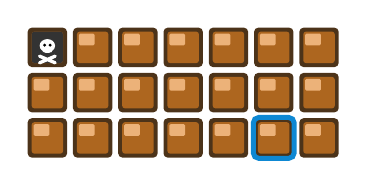
\begin{tikzpicture}[scale=0.5]
                    % チョコレートのマスを描画
                    \foreach \x in {0,...,6} {
                        \foreach \y in {0,...,2} {
                            % 外枠（暗い茶色）
                            \fill[brown!40!black, rounded corners=1.5pt]
                                (\x*1.15, -\y*1.15) rectangle ++(1.0, -1.0);
                            % 内側（明るい茶色）
                            \fill[brown!60!orange!80!black, rounded corners=1pt]
                                (\x*1.15+0.1, -\y*1.15-0.1) rectangle ++(0.8, -0.8);
                            % ハイライト（上面の光沢）
                            \fill[brown!50!orange!60!white, rounded corners=0.5pt]
                                (\x*1.15+0.15, -\y*1.15-0.15) rectangle ++(0.4, -0.3);
                        }
                    }
                    % 毒マス（左上）— 黒背景にドクロ
                    \fill[black!80, rounded corners=1pt]
                        (0.1, -0.1) rectangle ++(0.8, -0.8);
                    % ドクロ（TikZで描画）
                    \begin{scope}[shift={(0.5, -0.5)}, scale=0.28, white]
                        % 頭
                        \fill (0, 0.15) circle [x radius=0.7, y radius=0.6];
                        % 顎
                        \fill[rounded corners=1pt] (-0.4, -0.2) rectangle (0.4, -0.5);
                        % 目
                        \fill[black] (-0.25, 0.2) circle (0.15);
                        \fill[black] (0.25, 0.2) circle (0.15);
                        % 骨（クロス）
                        \draw[white, line width=1.2pt, line cap=round]
                            (-0.7, -0.8) -- (0.7, -1.4)
                            (0.7, -0.8) -- (-0.7, -1.4);
                        % 骨の端（丸）
                        \foreach \p in {(-0.7,-0.8),(0.7,-0.8),(-0.7,-1.4),(0.7,-1.4)} {
                            \fill[white] \p circle (0.12);
                        }
                    \end{scope}
                    % 選択マス（青枠）— 3行目6列目
                    \draw[cyan!70!blue, line width=1.8pt, rounded corners=2pt]
                        (5*1.15-0.02, -2*1.15+0.02) rectangle ++(1.04, -1.04);
                \end{tikzpicture}
            \end{column}
        \end{columns}
    \end{block}
\end{frame}

\begin{frame}{テーマについて}
    今回はChompというゲームを題材に「各プレイヤーがランダムに手を打つようなことを考えたら、どのような数学的特徴が見えるだろうか」という問いを立てて活動を行った。
\end{frame}